\documentclass[11pt]{article}
\usepackage[T1]{fontenc}
\usepackage[utf8]{inputenc}
\usepackage{lmodern,microtype}
\usepackage[a4paper,margin=25mm]{geometry}
\usepackage{amsmath,amssymb,amsthm,mathtools}
\usepackage{graphicx,booktabs,tabularx,listings,xcolor}
\usepackage[numbers,sort&compress]{natbib}
\usepackage[hidelinks,pdfauthor={Kun Huang},pdftitle={RoundGuard: Exact Attainable Discrepancies in Monetary Rounding Policies}]{hyperref}
\newtheorem{theorem}{Theorem}
\newtheorem{lemma}[theorem]{Lemma}
\newtheorem{proposition}[theorem]{Proposition}
\newcommand{\Q}{\mathsf{Q}}
\newcommand{\he}{\mathsf{he}}
\newcommand{\den}{\mathsf{den}}
\newcommand{\Z}{\mathbb Z}
\newcommand{\R}{\mathbb Q}
\lstset{basicstyle=\ttfamily\small,breaklines=true,columns=fullflexible,frame=single}
\title{RoundGuard: Exact Attainable Discrepancies\\in Monetary Rounding Policies}
\author{Kun Huang\\\small Economics and Management School, Wuhan University\\\small \texttt{huangkun123huang@163.com}}
\date{}
\newcommand{\DPCompleted}{72}
\newcommand{\ResidueCompleted}{35}
\newcommand{\SMTCompleted}{19}
\newcommand{\AutoMedian}{9.77}
\newcommand{\SMTMedian}{14.30}
\newcommand{\DPMaxMedian}{101.94}
\newcommand{\SmallNodesMin}{6}
\newcommand{\SmallNodesMax}{28}
\newcommand{\SmallDepthMin}{3}
\newcommand{\SmallDepthMax}{5}
\newcommand{\SmallVarsMin}{1}
\newcommand{\SmallVarsMax}{3}
\newcommand{\DPUnknown}{0}
\newcommand{\DPPartial}{0}
\newcommand{\DPTwoMedian}{1.49}
\newcommand{\DPFourMedian}{2.63}
\newcommand{\DPEightMedian}{10.28}
\newcommand{\DPSixteenMedian}{11.21}
\newcommand{\DPThirtyTwoMedian}{38.69}
\newcommand{\DPSixtyFourMedian}{101.94}
\newcommand{\ResidueUnknown}{25}
\newcommand{\ResiduePartial}{12}
\newcommand{\ResidueTwoMedian}{32.71}
\newcommand{\ResidueFourMedian}{81.83}
\newcommand{\ResidueEightMedian}{2024.58}
\newcommand{\ResidueSixteenMedian}{1765.17}
\newcommand{\ResidueThirtyTwoMedian}{1703.72}
\newcommand{\ResidueSixtyFourMedian}{1822.88}
\newcommand{\SMTUnknown}{36}
\newcommand{\SMTPartial}{17}
\newcommand{\SMTTwoMedian}{267.62}
\newcommand{\SMTFourMedian}{1953.54}
\newcommand{\SMTEightMedian}{1810.83}
\newcommand{\SMTSixteenMedian}{1574.38}
\newcommand{\SMTThirtyTwoMedian}{1606.18}
\newcommand{\SMTSixtyFourMedian}{1677.88}
\begin{document}
\maketitle
\begin{abstract}
Exact decimal arithmetic does not determine when a monetary calculation should be rounded. A line-item rule and its aggregate counterpart can produce different payable amounts even with exact rational intermediates. Universal rounding bounds do not determine whether their endpoints are attainable on permitted amount grids. We present RoundGuard, an exact analyzer for declared monetary rounding policies. Structural shifts reduce common-drift affine expressions to feasible representatives. For independent affine lines, a sufficient-state theorem retains attained residual extrema in at most two states: the parity of the summed rounded line outputs. Local-period enumeration followed by linear-time combination reconstructs inputs attaining both signed discrepancy endpoints, without a common-denominator residue product. Enumeration remains pseudo-polynomial in individual coefficient denominators; sign-sensitive modes require nonnegative raw lines or an unreduced satisfiability-modulo-theories (SMT) fallback. A JavaScript Object Notation (JSON) interface supports six rounding modes, finite placement families, and bounded piecewise expressions. Independent exhaustive decimal evaluation checks 66 small programs. Further experiments compare parity extrema, cyclic residue dynamic programming, reduced SMT, and full-grid SMT, including coprime-denominator cases. The contribution is a restricted sufficient-state analysis and reproducible implementation for feasible monetary discrepancies, using established periodic arithmetic and elementary parity optimization.
\end{abstract}

\section{Introduction}
Rounding stages are observable parts of a monetary rule. The UK HM Revenue \& Customs (HMRC) invoice guidance distinguishes line calculations from rounding the final value-added tax (VAT) total~\citep{hmrc_vat}. The US Internal Revenue Service (IRS) describes adjustments arising when payroll taxes are rounded during individual payroll computations~\citep{irs_p15}. US Social Security Administration (SSA) guidance prescribes different cent, dime, and dollar stages, and explicitly requires certain entitlement comparisons before lower-dollar rounding~\citep{ssa_rounding}. These examples concern specified discrete outcomes, not merely the numerical approximation of a real-valued formula.

The arithmetic foundation is already substantial. Fluctuat and Daisy analyze finite-precision computations, including fixed-point arithmetic~\citep{fluctuat2011,daisy2018}; FPTaylor derives rigorous roundoff bounds~\citep{fptaylor2015}. Catala gives executable legal specifications~\citep{catala2021}. Its date analysis proves insensitivity to alternative calendar rounding conventions~\citep{date2024}, while CUTECat encodes rational monetary rounding in Z3 and reports backend discrepancies~\citep{cutecat2025}. Therefore neither monetary rounding semantics nor counterexample generation alone constitutes the research gap addressed here.

Our narrower question is: \emph{what discrepancy can actually occur between declared monetary rounding policies on specified finite amount grids?} A universal bound treats operands as arbitrary rationals. A program's rates and permitted tick values can make extremal residuals impossible. Exhaustive evaluation is definitive but its input product grows with both the amount ranges and the number of lines. Generic exact integer reasoning can express the problem, but does not automatically exploit independent line structure.

We develop a specialized exact analysis with four components. First, structural shift certificates give a feasible representative domain for common-drift rounding policies. This instantiates established shift-periodic Chv\'atal and quasi-affine arithmetic~\citep{williams2011,basu_et_al2019,verdoolaege2010}; periodicity itself is not claimed as new. Second, a sufficient-state theorem identifies at most two parity states for attainable line-versus-total discrepancy extrema and provides witness reconstruction, including a nonnegative extension for sign-sensitive modes. Third, a runnable analyzer dispatches between this dynamic program, residue-reduced SMT, and unreduced bounded SMT. Fourth, an openly specified benchmark records independent oracles, executable diagnostics, and method ablations. The results characterize this restricted analyzer; they do not certify a deployed tax or payroll system.

\section{Examples and the analysis contract}
Amounts in the examples are measured in cents. Let $\Q_{q,m}$ round a rational to the zero-anchored grid $q\Z$ using mode $m$. With two raw line taxes $y_1=y_2=1/2$, nearest-even line rounding produces zero, whereas nearest-even total rounding produces one cent:
\[
 P_{\mathrm{line}}=\he(1/2)+\he(1/2)=0,
 \qquad P_{\mathrm{total}}=\he(1)=1.
\]
The distinction persists without binary floating-point arithmetic. Conversely, reassociating addition of values already on one exact monetary grid does not create rounding errors: every sum remains on that grid. RoundGuard includes this insensitive case rather than treating any rounded addition as a warning.

An input grid matters. The sharp nearest-even aggregation bound for an even number $n$ of arbitrary rational operands is $nq/2$. However, a line $y=x/5$ with integer $x$ cannot have a half-integer normalized value. Several such lines can prevent the universal extreme. A useful diagnostic must distinguish an unattainable envelope from a discrepancy reached by a valid input. The batch analysis retains feasible residues and returns an attaining assignment.

The user supplies a nonempty finite box of integer ticks, exact input quanta, and a finite family $\mathcal P$ of expression variants. The observation is the final rational amount, or a rational-valued branch result. We ask whether
\[
  \forall x\in X\;\forall P,Q\in\mathcal P,\quad P(x)=Q(x),
 \qquad
  \Delta(\mathcal P,X)=\max_{x\in X}\bigl(\max_{P\in\mathcal P}P(x)-\min_{P\in\mathcal P}P(x)\bigr).
\]
Completeness is relative to the supplied box and declared policy family. Optional sites enumerate round/no-round placements explicitly; RoundGuard does not infer whether a placement is legally admissible. A sensitive result does not select the correct policy or justify an automatic repair.

\section{Language and exact semantics}
The certified core consists of finite expressions
\[
\begin{gathered}
e ::= c\mid x_i\mid e+e\mid e-e\mid r e\mid \Q_{q,m}(e),\\
c,r\in\R,\quad q\in\R_{>0},\quad m\in\{\mathrm{FLOOR},\mathrm{CEILING},\mathrm{HALF\_EVEN}\}.
\end{gathered}
\]
An input is $s_i x_i$, where $x_i\in\Z$ and the declared positive rational $s_i$ is its quantum. Coefficients below are measured with respect to integer ticks, so they already include $s_i$. The interface labels grids as Money, Integer, Decimal, or Rate; Integer has unit quantum. These labels document input representation, rather than implement a currency or dimensional type system. Rates used in multiplication are exact constants. Products of two inputs, input-dependent divisors or quanta, overflow, and loops are unsupported.

For a normalized argument $t=y/q$, FLOOR and CEILING choose $\lfloor t\rfloor$ and $\lceil t\rceil$. HALF\_EVEN chooses a nearest integer, resolving a tie toward the even candidate. HALF\_UP follows the conventional decimal convention of nearest with ties away from zero. DOWN truncates toward zero; UP rounds away from zero. Multiplying the selected integer by $q$ gives the result. Rational constants are integers or strings such as \texttt{"0.062"} and \texttt{"1/3"}; JSON floating-point quanta and Python floating literals are rejected.

The implementation also supports \texttt{min}, \texttt{max}, and numeric conditionals with ordered comparisons. These are encoded exactly in bounded SMT but lie outside the general shift certificate. The following fragment generates the line and total variants automatically:
\begin{lstlisting}
{"variables": {"x": {"min": 0, "max": 19},
               "y": {"min": 0, "max": 19}},
 "batch": {"lines": ["x/5", "y/5"],
           "quantum": "1", "mode": "HALF_EVEN"}}
\end{lstlisting}
Expressions are parsed through Python's syntax tree, not executed as Python. Attribute access, arbitrary function calls, and nonlinear arithmetic are rejected. A JSON template can contain \texttt{maybe(e,q,m,site)}; shared site names make a correlated on/off decision, and distinct names enumerate independent choices. At most ten sites are enumerated. This is a finite policy interface rather than a source analyzer for arbitrary Python or Catala programs.

\section{Structural shifts and exact box reduction}
Erase each quantizer to obtain $\bar e(x)=b_e+\sum_i a_{e,i}x_i$. FLOOR and CEILING commute with integer grid shifts; nearest-even commutes with even grid shifts:
\begin{equation}\label{eq:translation}
 \Q_{q,m}(y+p_m kq)=\Q_{q,m}(y)+p_m kq,
 \qquad p_m=\begin{cases}1&m\in\{\mathrm{FLOOR},\mathrm{CEILING}\},\\2&m=\mathrm{HALF\_EVEN}.\end{cases}
\end{equation}
Both statements hold for negative $k$. An odd shift does not suffice for nearest-even: $\he(1/2)=0$ and $\he(3/2)=2$.

For every coordinate, inspect all quantizer nodes $v=\Q_{q_v,m_v}(u_v)$ in the family and define
\begin{equation}\label{eq:period}
 T_i=\mathop{\mathrm{lcm}}_v\den\!\left(\frac{a_{u_v,i}}{p_{m_v}q_v}\right).
\end{equation}
The denominator is reduced, and the empty lcm is one. These shifts are sufficient, not necessarily minimal.

\begin{proposition}[Common-drift reduction]\label{prop:period}
For a family in the certified core, every expression satisfies
$e(x+T_i\mathbf e_i)=e(x)+a_{e,i}T_i$.
If the variants have equal erased slope vectors, their pairwise differences are periodic with these coordinate periods. On $X=\prod_i\{L_i,\ldots,U_i\}$, all discrepancy values occur on
\[
 H=\prod_i\{L_i,\ldots,L_i+\min(T_i,U_i-L_i+1)-1\}.
\]
Every witness found on $H$ is feasible on $X$.
\end{proposition}
\begin{proof}
Constants and variables have their stated affine drift. Addition, subtraction, and constant scaling preserve it. At a quantizer, induction gives child drift $a_{u,i}T_i$. Equation~\eqref{eq:period} makes that drift a permitted multiple in~\eqref{eq:translation}; quantization preserves it. Subtracting two equal-slope drift identities yields periodic discrepancy. Map any coordinate to $L_i+((x_i-L_i)\bmod T_i)$. If the original width is smaller than $T_i$, this is the original coordinate; otherwise it lies in the first period. The mapped input lies in $H$, differs by period multiples, and preserves each discrepancy. Since $H\subseteq X$, the attainable value sets coincide.
\end{proof}

This proposition operationalizes known shift-periodic arithmetic, with explicit mixed-mode parity and feasible box representatives. It is not an efficiency guarantee for a general graph: $|H|$ can be a large product, and coefficient denominators can make $T_i$ large. Unequal slopes trigger unreduced SMT. HALF\_UP, DOWN, and UP also trigger that fallback: they do not have global signed translation covariance. For example, HALF\_UP maps $-1/2$ to $-1$ and $3/2$ to $2$, violating even-shift covariance across zero. Nonnegative inputs alone would be insufficient if a negative intermediate expression were permitted.

\section{Attainable extrema for independent lines}
Normalize a common quantum $q$ to one and let
\[
 y_i=a_i x_i+c_i,\quad x_i\in\{L_i,\ldots,U_i\},\qquad
 P_{\mathrm{total}}=R_0\!\left(\sum_i y_i\right),\quad
 P_{\mathrm{line}}=\sum_i R_i(y_i).
\]
Each line has its own independent tick input. Constant lines are allowed. The theorem permits local and outer FLOOR, CEILING, or HALF\_EVEN modes; the implementation uses one common mode and rejects repeated line-input dependencies.

Define rounded integers $k_i=R_i(y_i)$ and residuals $f_i=y_i-k_i$, with $K=\sum_i k_i$ and $F=\sum_i f_i$. Then
\[
 P_{\mathrm{total}}-P_{\mathrm{line}}=R_0(K+F)-K.
\]
Integer covariance removes $K$ for outer FLOOR or CEILING. For HALF\_EVEN only $\kappa=K\bmod2$ remains. The monotone terminal functions are
\[
 g_\kappa(F)=\he(F+\kappa)-\kappa\quad\text{(HALF\_EVEN)},\qquad
 g(F)=\lfloor F\rfloor\ \text{or}\ \lceil F\rceil.
\]
Parity is necessary: lines $y_1=1/2$ and $y_2=x$, $x\in\{0,1\}$, have the same $F=1/2$ but discrepancies zero and one.

A sufficient local shift is $T_i=\den(a_i/2)$, including $T_i=1$ for a constant line. It changes $y_i$ by an even integer, preserving $f_i$ and $k_i\bmod2$. Enumerate the first $m_i=\min(T_i,U_i-L_i+1)$ feasible ticks. For each attainable local parity $b$, retain the minimum $\ell_i(b)$ and maximum $u_i(b)$ of $f_i$, with attaining ticks. For an outer FLOOR or CEILING collapse the parity classes to one state. The offset $c_i$ affects values but does not affect this sufficient period.

For nearest-even initialize only $V_0^-(0)=V_0^+(0)=0$ and update reachable states by
\begin{align}
 V_j^-(\kappa)&=\min_{s\oplus b=\kappa}\bigl(V_{j-1}^-(s)+\ell_j(b)\bigr),\label{eq:dpmin}\\
 V_j^+(\kappa)&=\max_{s\oplus b=\kappa}\bigl(V_{j-1}^+(s)+u_j(b)\bigr),\label{eq:dpmax}
\end{align}
where $\oplus$ denotes exclusive-or. In the one-state case simply sum local extrema. Retained endpoints are attained; intermediate residuals need not be attainable.

\begin{theorem}[Exact batch discrepancy]\label{thm:dp}
Under the independent affine-line premises, for outer HALF\_EVEN the exact signed extrema are
\begin{align*}
 \delta_{\min}&=\min_{\kappa\ \mathrm{reachable}}g_\kappa(V_n^-(\kappa)),&
 \delta_{\max}&=\max_{\kappa\ \mathrm{reachable}}g_\kappa(V_n^+(\kappa)).
\end{align*}
For outer FLOOR or CEILING apply $g$ to the one-state minimum and maximum. Both endpoints have reconstructible in-box inputs. Equivalence holds exactly when both are zero. The largest absolute discrepancy is $\max(|\delta_{\min}|,|\delta_{\max}|)$. Multiply by $q$ to recover monetary units.
\end{theorem}
\begin{proof}
Even translation preserves each local residual and parity, so feasible representatives preserve every relevant local pair. Induct on prefix length. A feasible prefix splits into a previous prefix and a local choice; independence permits every such pair to combine. At a fixed parity decomposition attained residual extrema add. Optimizing over decompositions proves~\eqref{eq:dpmin}--\eqref{eq:dpmax} and attainment.

Write $K=2h+\kappa$. Even covariance gives $\he(K+F)-K=g_\kappa(F)$; integer covariance gives $g(F)$ for FLOOR and CEILING. Each terminal function is nondecreasing, so its extrema at a fixed state occur at the retained residual endpoints. Taking extrema over reachable states proves the formulas. A predecessor state and local tick at each retained endpoint reconstruct a feasible assignment attaining it.
\end{proof}

Local enumeration and combination use $O(\sum_i m_i+n)$ arithmetic operations, constant working values, and $O(n)$ backpointer records. Reconstruction costs $O(n)$. These bounds exclude rational operand bit costs. An individual $T_i$ can be exponential in its binary coefficient description, so this enumeration implementation is pseudo-polynomial. The prototype declines the path if any $m_i>400$; short intervals remain supported even when $T_i>400$. No common-denominator residue table is constructed; rational prefix sums can still have growing denominator bit lengths.

An ablation retains a larger cyclic-residue algorithm. With a common denominator $B$ and modulus $M=2B$, it tracks raw-sum residue and additive rounding-error extrema, then evaluates the outer error at each reachable residue. It also yields exact attained endpoints, but dense combination costs $O(nM^2)$ and the prototype caps $M$ at 400. Its full proof is in the artifact ledger. The parity theorem identifies information unnecessary for this objective. The additive two-state recurrence is elementary and can alternatively be implemented by independent choices plus a least-cost parity correction.

\begin{proposition}[Nonnegative sign-sensitive extension]\label{prop:positive}
Theorem~\ref{thm:dp} extends to HALF\_UP, DOWN, and UP when each raw normalized line is nonnegative on its declared interval.
\end{proposition}
\begin{proof}
On nonnegative raw arguments these modes equal $\lfloor t+1/2\rfloor$, $\lfloor t\rfloor$, and $\lceil t\rceil$. Local representatives remain in their original domains, so local residual enumeration is valid. The actual raw total $K+F$ is nonnegative; its rounded discrepancy is respectively $\lfloor F+1/2\rfloor$, $\lfloor F\rfloor$, or $\lceil F\rceil$. These monotone extended terminal functions remain valid for negative $F$ and need no parity state. Independence and attainment follow as before.
\end{proof}
Applying the signed HALF\_UP, DOWN, or UP operator directly to $F$ would be incorrect. A nonnegative $y=1/5$ rounded UP has $F=-4/5$; an outer DOWN discrepancy is $\lfloor F\rfloor=-1$, whereas signed truncation of $F$ gives zero. The implementation checks affine endpoint values of every raw line. Otherwise it falls back. A fixed grand total or shared discount input requires coupled reasoning; the batch interface does not support such constraints.

\section{SMT fallback and diagnostic guarantees}
We encode integer input ticks, rational arithmetic, floor casts, tie comparisons, and integer parity in Z3~\citep{z32008}. An expression has a statically fixed rational output denominator: addition takes an lcm, constant scaling multiplies denominator bounds, and a quantizer returns an integer times its quantum. Therefore multiplying a discrepancy by a common denominator gives an integer objective.

The analyzer first asks whether any pair differs. UNSAT yields SAFE within the declared scope. SAT yields a concretely replayed witness. For exact extrema, it binary-searches the nonnegative integral family spread between an attained lower bound and a sound upper envelope. For common full erasures, propagated absolute quantization errors give an envelope; otherwise ordinary rational range intervals do. Each successful threshold query supplies a model. Completed search supplies an optimum with a replayed attaining input. A solver timeout produces UNKNOWN for detection, or SENSITIVE with unestablished maximum and valid lower/upper bounds after a witness has already been found. Neither is reported as an equivalence proof or an exact optimum.

\begin{proposition}[Conditional analyzer correctness]\label{prop:sound}
Assuming the implemented concrete and symbolic operators agree with the stated semantics, and successful solver answers are correct, every completed SAFE result implies equality of the declared variants over the input box. Every completed maximum is the attainable family spread on that box. The DP path requires the premises of Theorem~\ref{thm:dp} or Proposition~\ref{prop:positive}; the reduced SMT path requires Proposition~\ref{prop:period}.
\end{proposition}
\begin{proof}
Residue reduction preserves discrepancy value sets, while the batch DP preserves their attained extrema and the zero-discrepancy test. An unreduced SMT query is the direct counterexample formula for the finite box. After a SAT query, a sound upper bound and integer objective make threshold feasibility monotone; binary search terminates at the largest feasible objective. Replaying its model establishes attainment. UNSAT on the difference formula establishes equality. Unknown queries do not justify either conclusion.
\end{proof}
This is an algorithmic argument under implementation and solver assumptions, not a mechanized verification of Python or Z3. The proof ledger labels mathematical results PROVED and executable enumeration as bounded sanity checks. No result is labelled MACHINE-CHECKED by a proof assistant.

\section{Evaluation}
\label{sec:evaluation}
\paragraph{Questions, corpus, and protocol.}
We ask whether completed diagnostics agree with independently executed small-grid semantics, whether residue reduction and the specialized DP change exact-search behavior, and whether a universal envelope is attained on the declared grids. The deterministic generator uses seed 20261003. The effectiveness corpus contains 48 synthetic programs, 12 canonical examples, and six public-rule-derived fragments: 66 programs in total, of which the oracle classifies 50 as sensitive and 16 as safe. The corresponding group counts are 37/48, 8/12, and 5/6 sensitive. Each program has \SmallVarsMin{}--\SmallVarsMax{} tick variables, two to four policies, and 21--1600 input assignments. Counting repeated syntax separately across policies gives \SmallNodesMin{}--\SmallNodesMax{} abstract syntax tree (AST) nodes (median 13); maximum root-to-leaf depth is \SmallDepthMin{}--\SmallDepthMax{} (median 4), with the root counted as depth one. These are small expression benchmarks rather than production programs.

The exhaustive oracle evaluates all 19,940 assignments in this corpus using Python Decimal's six rounding conventions, separately from the analyzer's Fraction quantizer and SMT encoding. Terminating rationals are converted by exact digit-tuple construction, independent of Decimal's current precision. The precision budget includes denominator powers of two and five and intermediate decimal spans. Inexact and rounded arithmetic traps reject silent approximation; only the explicitly requested grid quantization may round. Nonterminating conversions or normalized quantum divisions are rejected. All saved corpus computations complete under these guards. The oracle shares the parsed AST with the analyzer, so this agreement tests arithmetic and analysis after parsing; it does not independently establish every parser translation. Saved \texttt{ground\_truth.json} records each oracle maximum and witness, and \texttt{diagnostics.json} records method outputs.

RoundGuard's automatic dispatch is compared with the same symbolic encoder on the full box, 32 uniformly sampled assignments, Hypothesis search configured with \texttt{max\_examples=64}, and independent range intervals for each policy. Sampling stops at the first differing assignment; Hypothesis may also shrink a found example, so 64 is a configuration parameter rather than a matched wall-time or strict total-evaluation budget. A testing result with no witness does not prove equality. Interval warnings are counted against the exact label, but the interval baseline is a deliberately simple correlation-losing envelope, not a state-of-the-art numerical analyzer. The effectiveness measurements have one execution per program and method; their medians summarize this heterogeneous corpus rather than repeated-run timing uncertainty.

\paragraph{Small-grid agreement and detection.}
\begin{table}[ht]
\centering\begin{tabular}{lrrrrr}
\toprule
Method & Cases & FP & Missed & Unknown & Median ms \\
\midrule
RoundGuard & 66 & 0 & 0 & 0 & 4.32 \\
Full-grid SMT & 66 & 0 & 0 & 0 & 5.92 \\
Random (32) & 66 & 0 & 2 & 0 & 1.00 \\
Hypothesis (64) & 66 & 0 & 1 & 0 & 45.82 \\
Independent intervals & 66 & 15 & 0 & 0 & 0.13 \\
\bottomrule
\end{tabular}
\caption{Effectiveness on 66 programs: 50 sensitive and 16 safe. FP (false positive) counts warnings on oracle-safe programs; Missed counts oracle-sensitive programs without a reported witness or warning. A testing miss is not a false proof of safety. Exact-method maxima also agree with the exhaustive oracle. Median wall times are across programs.}
\label{tab:accuracy}
\end{table}
Both exact methods complete on all 66 programs, match every oracle maximum, and have no false warnings or missed sensitive cases (Table~\ref{tab:accuracy}). Automatic dispatch selects residue DP for 22 programs, reduced SMT for 19, and unreduced SMT for 25. Its median wall time is \AutoMedian\,ms, compared with \SMTMedian\,ms for full-grid SMT. Random testing misses two threshold programs, and Hypothesis misses one currency-conversion program. Independent intervals warn on 15 of the 16 safe programs. These results establish agreement on the saved cases; neither the mixture nor the small miss counts estimates defect prevalence in financial software.

\paragraph{Scaling and method ablations.}
The scaling suite has 24 independent-line cases: $n\in\{2,4,8,16,32,64\}$, tick bounds $0\le x_i\le U$ with $U\in\{3,20,10^4,10^9\}$, and cyclic rates $1/2,1/4,1/5,1/10$. All use cent HALF\_EVEN rounding. The modulus is $M=8$ for two lines and $M=40$ otherwise; this suite varies line count and amount-window width, not large coefficient denominators. The largest box contains $(10^9+1)^{64}$ assignments. We execute each case and each of DP, reduced SMT, and full-grid SMT three times, giving 216 saved runs. Reduced versus full SMT isolates structural box reduction within one encoder; reduced SMT versus DP evaluates the additional independent-line recurrence.

All methods are timed from analysis entry through the returned diagnostic with \texttt{perf\_counter}; JSON loading and oracle construction are excluded, while method-specific preprocessing, encoding, optimization, and replay are included. The solver limit is 1500\,ms \emph{per check}, including the initial detection check and each binary-search query. Consequently a complete or partially optimized run can take longer than 1.5\,s. This is not an equal total-run budget, and the DP has no matching timeout. Measurements come from one Windows machine with Python 3.11.5 and Z3 4.15.3; package versions and protocol settings are saved in \texttt{environment.json}.

DP establishes the exact maximum in \DPCompleted/72 runs, reduced SMT in \ResidueCompleted/72, and full-grid SMT in \SMTCompleted/72. Among unfinished reduced-SMT runs, \ResidueUnknown{} return UNKNOWN before finding a witness and \ResiduePartial{} report sensitivity with an unestablished maximum. The corresponding full-grid counts are \SMTUnknown{} and \SMTPartial{}. Both outcomes are distinct from either a proof of equality or an exact optimum, and their separate statuses remain in the raw records.

\begin{figure}[ht]
\centering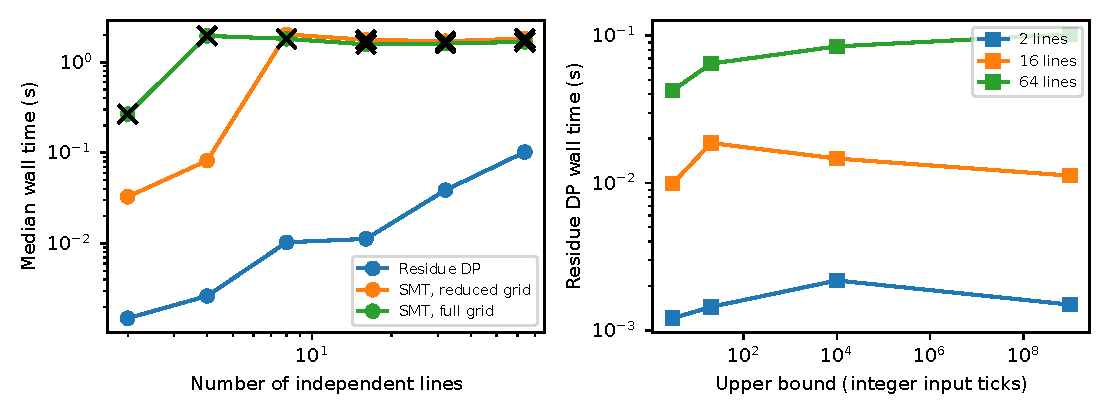
\includegraphics[width=\linewidth]{figures/scalability.pdf}
\caption{Saved scaling measurements. Left: median observed wall time over three runs at $U=10^9$; a cross marks a cell with at least one unfinished optimum computation. Such points measure time to the returned diagnostic and must not be interpreted as time to an exact answer. Right: DP timing as amount-window width changes for selected line counts. Coefficient denominators remain fixed within these curves.}
\label{fig:scaling}
\end{figure}

The largest DP median over the 24 cases is \DPMaxMedian\,ms (Figure~\ref{fig:scaling}). For the four-line, $U=10^9$ cell, the SMT medians are \ResidueFourMedian\,ms with structural reduction and \SMTFourMedian\,ms on the full grid. Reduction is not guaranteed to improve solver wall time: encoding and solver overhead can change its practical effect. Cells containing unfinished runs do not support exact-answer speedup ratios. The DP's finite residue work explains its weak dependence on interval width here, while larger denominators, coupled inputs, or branch structure require separate evaluation. Runtime and completion numbers are generated from the saved records through \texttt{result\_macros.tex}; reruns on another machine require reexamining the resulting plot and outcomes.

\paragraph{Independent scaling certificates and bound quality.}
Large boxes are not exhaustively enumerated. For each line, an independently executed Decimal table covers its feasible local period, or its whole interval when shorter; the sufficient periods of these benchmark rates are at most 20 ticks. Summing the local error minima and maxima gives a sound envelope for the total line error. The outer nearest-rounding error is at most $1/2$ cent. Since the final discrepancy is an integer number of cents, flooring this envelope supplies an independent integral upper bound. A DP-produced input is checked against every declared tick bound and replayed through Decimal. Its attained spread equals that independently derived upper bound in all 24 cases, certifying the maximum without assuming the DP's optimum calculation. The certificate values and witnesses are saved in \texttt{scaling\_ground\_truth.json}. This construction is specific to the saved scaling family, not an independent solver for arbitrary input programs.

The unrestricted nearest-even envelope is $\he(n/2)$ cents. At 64 lines and $U=3$, RoundGuard finds an attainable maximum of 27 cents, compared with the universal 32-cent envelope. At $U\ge20$, the 64-line maximum is 30 cents, leaving a two-cent gap even with complete local-period coverage; the heterogeneous line grids still exclude the universal endpoint. For 32 lines the corresponding maxima are 14 and 15 cents, compared with 16 cents universally. The saved upper-envelope certificate is tight in all scaling cases, whereas the universal envelope is strictly larger in ten of the 24 cases. This difference measures attainable-bound precision on declared grids, rather than a change in rounding semantics.



\section{Public-rule-derived fragments}
\label{sec:cases}
The benchmark includes independently written fragments motivated by publicly documented rounding stages. They are deliberately small and contain explicit counterfactual policies; they are not complete legal calculators. Table~\ref{tab:cases} gives the attained spread on the grids saved in each JSON file.
\begin{table}[ht]
\centering\begin{tabular}{lrl}
\toprule
Fragment & Maximum (cents) & Method \\
\midrule
cash\_settlement & 5 & residue-dp \\
hmrc\_invoice & 0 & residue-smt \\
irs\_payroll & 1 & smt \\
rational\_money & 1 & smt \\
ssa\_benefit & 66 & residue-smt \\
ssa\_entitlement & 50 & smt \\
\bottomrule
\end{tabular}
\caption{Exact discrepancy on six rule-derived fragments. Values are cents. A difference establishes sensitivity of the stated comparison, not a defect in the cited rule or deployed software.}\label{tab:cases}
\end{table}

The HMRC fragment compares line VAT rounded down to tenths of a penny, followed by final penny rounding, with final-only penny rounding~\citep{hmrc_vat}. The two-line 20\% rate and narrow amount windows are benchmark assumptions, not an assertion that every policy applies to every trader. Payroll uses the separate 6.2\% and 1.45\% employee-side rates appearing in the IRS fractions-of-cents discussion and compares them with a deliberately combined-rate calculation~\citep{irs_p15}. It ignores wage caps, Additional Medicare Tax, and reporting adjustments. Shared wages make this a coupled expression, handled by SMT rather than independent-line DP.

The benefit fragments isolate the SSA's prescribed dime/dollar stages and the order of entitlement comparison~\citep{ssa_rounding}; the chosen adjustment factor, offset, and entitlement threshold are illustrative inputs, not a full statutory benefit formula. Cash settlement compares final nickel rounding with an intentionally early per-component alternative motivated by Canadian guidance to round the final bill after taxes~\citep{cra_cash}. The software fragment compares an intermediate-rounded rational calculation with deferred rounding, motivated by Brick Money's documented RationalMoney workflow~\citep{brick_money}. Its rates are independently chosen, and no external implementation is copied.

\section{Related work}
Skala's non-peer-reviewed preliminary draft studies consistent rounding of financial totals~\citep{skala2017}. It gives algorithms to choose rounded labels for a fixed totals forest, including minimax node-error optimization. Its line-versus-total motivation is directly adjacent to ours. RoundGuard instead fixes the policies and optimizes their discrepancy over permitted input grids; the different objective makes Skala's algorithms unsuitable as same-task runtime baselines.

Aswal et al. analyze financial decimal operations on binary machines and construct transaction sequences with persistent rounding differences~\citep{aswal2012}. Their error tables compare binary execution with correctly rounded decimal operations. Our question instead compares prescribed exact policies over bounded feasible input grids, with no binary-versus-decimal representation discrepancy.

Shift-periodic nested rational ceiling expressions already appear in Williams' account of Chv\'atal functions~\citep{williams2011}. Basu et al. formalize affine Chv\'atal trees and mixed-integer representability~\citep{basu_et_al2019}. The isl library manipulates exact integer sets and quasi-affine expressions~\citep{verdoolaege2010}; Presburger functions and counting have broader structural treatments~\citep{woods2015}. RoundGuard specializes these foundations to feasible representatives for prescribed monetary policies. It does not offer a new decidability result or a general competitor to integer-set libraries.

The larger cyclic ablation belongs to the established min/max-plus dynamic-programming pattern; the two-state optimization is simpler still. Work on near-convex min-plus convolution accelerates structured knapsack instances~\citep{bringmann_cassis2023}; our residue tables need not satisfy those additional premises, and the prototype uses direct sparse convolution. Low-discrepancy sequence rounding also uses compact state graphs and optimization~\citep{sadakane2001}. It chooses rounded outputs for a fixed sequence, whereas our batch formulation fixes rounding policies and optimizes over feasible amount grids. This distinction limits the claimed application-specific contribution.

Numerical analyzers such as Fluctuat, Daisy, FPTaylor, and Gappa provide sound error analysis or certificates~\citep{fluctuat2011,daisy2018,fptaylor2015,gappa2010}. Fixed-point synthesis studies implementation accuracy~\citep{fixedpoint2013}; Flocq supplies foundational arithmetic proofs~\citep{flocq2011}. Herbie searches expression rewrites using sampled accuracy estimates~\citep{herbie2015}, and robustness analyses handle discontinuous branch changes~\citep{robust2013}. These systems address richer numerical programs than our exact affine batch fragment. RoundGuard's different contract is an attained discrepancy between two prescribed discrete policies, rather than an approximation guarantee against an ideal real formula.

Catala's semantics and verified compilation address translating computational law~\citep{catala2021}; the date work already treats rounding-insensitivity as a relational property~\citep{date2024}. CUTECat's rational monetary encoding and backend discrepancy findings are direct prior art for our fallback and motivation~\citep{cutecat2025}. Recent recommendations for public administrations likewise emphasize exact monetary representation and testing~\citep{codinglaws2026}. The present work adds a restricted attainable-extrema path, and provides no Catala integration. FPBench motivates auditable benchmarks for numerical tools~\citep{fpbench2017}; our JSON monetary suite is separate and is not claimed as an extension of FPBench.

\section{Limitations and validity}
The main risk to practical generalization is independence. Many payroll and benefit computations share input amounts, use piecewise bands, or constrain an invoice's grand total. Those programs use the bounded fallback, or require constructs outside this implementation. The prototype supports only one active tick variable per affine DP line and one common rounding mode, despite the theorem allowing different covariant local modes. Generic optional placements are explicitly enumerated rather than compressed by the batch theorem. The pseudo-polynomial enumeration cost is an implementation property, not a lower bound for the independent-line problem. For fixed local parity, write $k_i=2t+b$; the rounded residual constraints and linear objective form a two-variable integer program in $x_i,t$. Rational strict endpoints can be converted to integer inequalities. Fixed-dimensional integer programming admits polynomial-time algorithms~\citep{lenstra1983}, suggesting an alternative local optimizer that this prototype does not implement. Large denominators can eliminate the DP advantage; full-period enumeration is not polynomial in coefficient bit size.

The evaluation is a controlled microbenchmark study on one Windows machine. Its generated amounts are not sampled transaction data, and the six public-rule-derived cases are simplified fragments. The suite demonstrates consistency against independent exact oracles, not prevalence of defects in financial software. Both SMT paths share the same encoder, so their comparison isolates domain reduction and batch structure rather than ranking independently developed solvers. Timeouts are per check, and do not create one equal total-run budget. Runtime depends on solver version, scheduling, and machine load; seeds fix inputs and search configuration but cannot fix wall time.

The mathematical proofs are ordinary proofs independently reviewed for their premises. Enumeration and property tests provide additional bounded checks; they cannot substitute for a proof. Decimal oracle comparisons share the parsed tree and therefore do not independently validate the parser's entire translation. Parser rejection and known-output integration tests mitigate part of that risk. Source rules were read on the stated research date; rule changes require revisiting the fragments. No diagnostic decides legal compliance, chooses a preferred policy, or verifies the author's institutional software.

\section{Conclusion}
RoundGuard computes feasible rounding-policy discrepancies in a deliberately restricted exact monetary model. Structural periods reduce amount grids when drift cancels, while a parity-conditioned extrema calculation avoids multiplying independent line domains. The analysis returns attained extrema and concrete witnesses, with explicit parity, sign, independence, and denominator conditions. The implementation and benchmark make those conditions observable and route unsupported cases to bounded SMT. Extending the useful batch path to coupled domains and validating it on larger source programs remain open work.

\paragraph{Availability and assistance.}
Code, inputs, results, proofs, and reproduction scripts are available at \url{https://github.com/beibeihk/roundguard}. AI tools assisted literature triage, implementation, and manuscript drafting. Reported computations have executable artifact records; the proofs are not proof-assistant mechanizations.

\bibliographystyle{plainnat}
\bibliography{references}
\appendix
\section{A sharp aggregation envelope}
\begin{lemma}\label{lem:sharp}
For arbitrary rational operands $y_1,\ldots,y_n$ on a shared quantum $q$, the largest absolute nearest-even line/total discrepancy is $q\he(n/2)$. For FLOOR or CEILING it is $(n-1)q$.
\end{lemma}
\begin{proof}
Normalize $q=1$. For floor, write $y_i=k_i+f_i$ with $0\le f_i<1$. The signed line-minus-total discrepancy is $-\lfloor\sum_i f_i\rfloor$, ranging from $-(n-1)$ to zero. Rational fractions sufficiently near one attain the lower endpoint. Ceiling follows by negation.

For nearest-even set $k_i=\he(y_i)$ and $f_i=y_i-k_i\in[-1/2,1/2]$. If $|f_i|=1/2$, $k_i$ is even. Put $K=\sum_i k_i$, $F=\sum_i f_i$. The discrepancy is $K-\he(K+F)$. If $n=2h$, $|F|\le h$ and nearest rounding cannot select an integer beyond $K\pm h$. If $n=2h+1$, the strict interior $|F|<h+1/2$ gives absolute discrepancy at most $h$. At either boundary, all local residuals are the same half tie, so $K$ is even; the outer tie gives $h$ if $h$ is even and $h+1$ if $h$ is odd. This is exactly $\he(n/2)$. Choosing every operand $1/2$, or every operand $-1/2$, attains the endpoints. Rescale by $q$.
\end{proof}
This elementary envelope is included for comparison, not as a novelty claim. Restricted input grids can give strictly smaller attainable extrema.
\end{document}



